%
% Annual Cognitive Science Conference
% Sample LaTeX Paper -- Proceedings Format
%

% Original : Ashwin Ram (ashwin@cc.gatech.edu)       04/01/1994
% Modified : Johanna Moore (jmoore@cs.pitt.edu)      03/17/1995
% Modified : David Noelle (noelle@ucsd.edu)          03/15/1996
% Modified : Pat Langley (langley@cs.stanford.edu)   01/26/1997
% Latex2e corrections by Ramin Charles Nakisa        01/28/1997
% Modified : Tina Eliassi-Rad (eliassi@cs.wisc.edu)  01/31/1998
% Modified : Trisha Yannuzzi (trisha@ircs.upenn.edu) 12/28/1999 (in process)
% Modified : Mary Ellen Foster (M.E.Foster@ed.ac.uk) 12/11/2000
% Modified : Ken Forbus                              01/23/2004
% Modified : Eli M. Silk (esilk@pitt.edu)            05/24/2005
% Modified : Niels Taatgen (taatgen@cmu.edu)         10/24/2006
% Modified : David Noelle (dnoelle@ucmerced.edu)     11/19/2014

%% Change "letterpaper" in the following line to "a4paper" if you must.

%%% MAX = 6 Pages (including references)

\documentclass[10pt,letterpaper]{article}

\usepackage{cogsci}
\usepackage{pslatex}
\usepackage{graphicx}
\usepackage{apacite}
\usepackage{color}


\title{Word Identification Under Multimodal Uncertainty}

\author{{\large \bf Abdellah Fourtassi} \\ afourtas@stanford.edu \\
  Department of Psychology\\ Stanford University\\
  \And {\large \bf Michael C. Frank}\\ mcfrank@stanford.edu \\
  Department of Psychology\\ Stanford University}


\begin{document}

\maketitle


\begin{abstract}

Identifying the visual referent of a spoken word -- that a particular insect is referred to by the word ``bee'' -- requires both the ability to process and integrate multi-modal input and the ability to reason under uncertainty. How do these tasks interact with one another? We introduce a task that allows us to examine how adults identify words under joint uncertainty in the auditory and visual modalities. We propose a ideal observer model of the task which provides an optimal baseline. Model predictions are tested in two experiments where word recognition is made under two kinds of uncertainty: category ambiguity and distorting noise. In both cases, the ideal observer model explains much of the variance in human judgments. But when one modality had noise added to it, human perceivers systematically preferred the unperturbed modality to a greater extent than the ideal observer model did.

\textbf{Keywords:}
Language; audio-visual processing; word learning; speech perception; computational modeling.
\end{abstract}


Language uses symbols expressed in one modality (e.g., the auditory modality, in the case of speech) to communicate about the world, which we perceive through many different sensory modalities. Consider hearing someone yell ``bee!" at a picnic, as a honeybee buzzes around the food. Determining reference involves processing the auditory information and linking it with other perceptual signals (e.g., the visual image of the bee, the sound of its wings, the sensation of the bee flying by your arm).

This multi-modal integration task takes place in a noisy world. On the auditory side, individual acoustic word tokens are almost always ambiguous with respect to the particular sequence of phonemes they represent, which is due to the inherent variability of how a phonetic category is realized acoustically \cite<e.g.,>{hillenbrand1995}. And some tokens may be distorted additionally by mispronunciation or ambient noise. Perhaps the speaker was yelling ``pea" and not ``bee.'' Similarly, a sensory impression may not be enough to make a definitive identification of a visual category.\footnote{In the general case, language can of course be visual as well as auditory, and object identification can be done through many modalities. For simplicity, we focus on audio-visual matching here.} Perhaps the insect was a beetle or a fly instead.

Thus, establishing reference requires reasoning under a great deal of uncertainty in both modalities. The goal of this work is to characterize such reasoning.  Imagine, for example, that someone is uncertain whether they heard ``pea" or ``bee'', does it make them rely more on the visual modality (e.g., the object being pointed at)? Vice versa, if they are not sure if they saw a bee or a fly, does that make them rely more on the auditory modality (i.e., the label)? More importantly, when input in both modalities is uncertain to varying degrees, do they weight each modality according to its relative reliability, or do they over-rely on a particular modality?

In this paper, we propose a probabilistic framework where such reasoning can be expressed precisely. We characterize uncertainty in each modality with a probability distribution, and we predict ideal responses by combining these probabilities in a optimal way. Our work can be seen as an extension to previous Bayesian models of phoneme identification \cite<e.g.,>{feldman2009}, where, instead of a unimodal input, we model a bimodal one. A few studies have explored some aspects of audio-visual processing in a probabilistic framework  \cite{bejjanki2011, kleinschmidt2015}. In these studies, the researchers focused on the specific case of phoneme recognition from speech and lip movement, however, where information is tightly correlated across modalities.

In the present work, we study, rather, the case of arbitrary mapping between sounds and visual objects. We test participants on their ability to process audio-visual stimuli and use them to recognize the underlying word. More precisely we study the case where both the word's form and the word's referent are ambiguous, and we examine the extent to which humans conform to, or deviate from the predictions of the ideal observer model. Moreover, some previous studies on audio-visual processing documented cases of modality preference, when people rely predominantly on the visual modality \cite<e.g., >{colavita1974} or the auditory modality \cite<e.g., >{sloutsky2003}. Thus, we will explore if participants in our task show evidence of a modality preference.

The paper is organized as follows. First, we introduce our audio-visual recognition task. We next present the ideal observer model. Then we present two behavioral experiments where we test word recognition under audio-visual uncertainty. In Experiment 1, audio-visual tokens are ambiguous with respect to their category membership. In Experiment 2, we intervene by adding  noise to one modality. In both experiments participants show qualitative patterns of optimal behavior. Moreover, while participants show no modality preference in Experiment 1, in Experiment 2 they over-rely on visual input when the auditory modality is noisy.

\section{The Audio-Visual Word Recognition Task}

We introduce a new task that tests audio-visual word recognition. We use two visual categories (cat and dog) and two auditory categories (/b/ and /d/ embedded in the minimal pair /aba/-/ada/). For each participant, an arbitrary pairing is set between the auditory and the visual categories, leading to two audio-visual word categories (e.g., dog-/aba/, cat-/ada/).

In each trial, participants are presented with an audio-visual target (the prototype of the target category), immediately followed by an audio-visual test stimulus (Figure \ref{fig:task}). The test stimulus may differ from the target in both the auditory and the visual components.  After these two presentations, participants press ``same'' or ``different.''

This task is similar to the task introduced by \citeA{sloutsky2003} and used in subsequent research to probe audio-visual encoding. However, unlike this previous line of research, here participants are not asked whether the two audio-visual presentations are identical. Instead, the task is category-based: They are asked to press `same' if they think the second item (the test) belonged to the same category as the first (target) (e.g.,  dog-/aba/), even if there is a slight difference in the word, in the object, or in both. They are instructed to press `different' only if they think that the second stimulus was an instance of the other word category (cat-/ada/).

The task also included trials where pictures were hidden (audio-only) or where sounds were muted (visual-only). These unimodal trials provide us with participants' categorization functions for the auditory and visual categories and are used as inputs to the ideal observer model, described below.

\begin{figure}[tp]
\centering
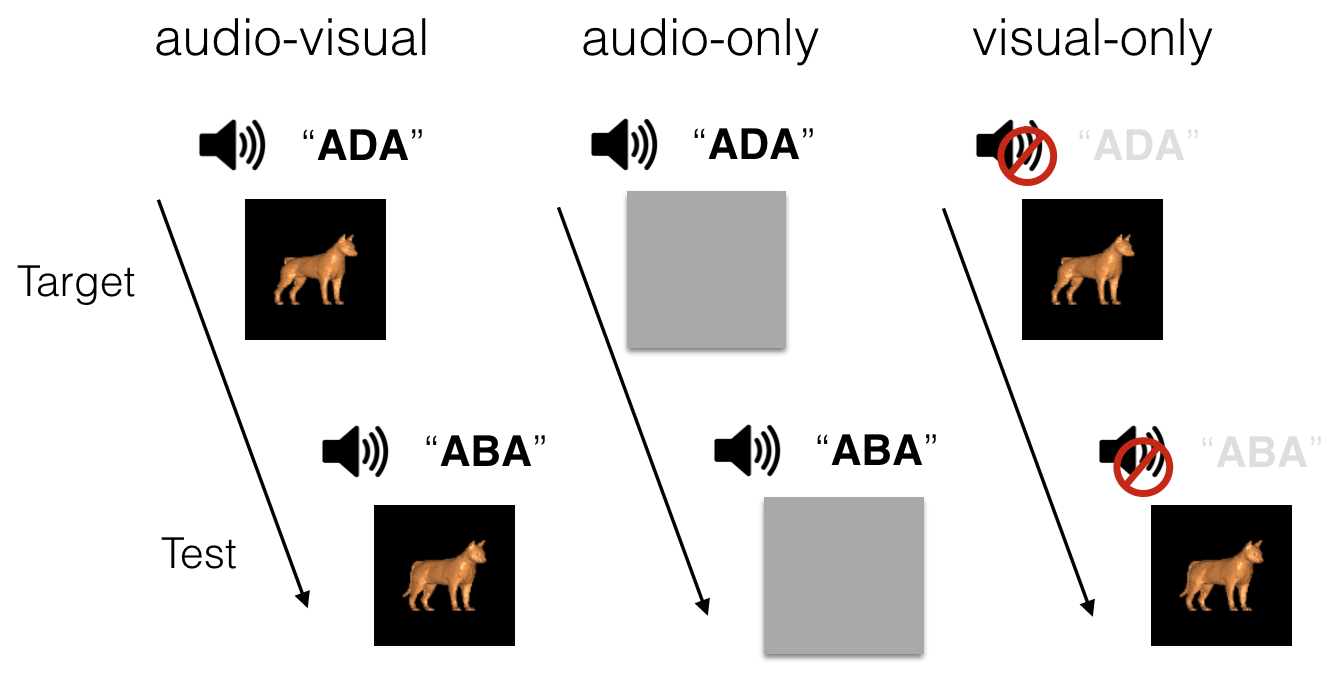
\includegraphics[width=0.4\textwidth]{task1.png}
\caption{Overview of the task}
\label{fig:task}
\end{figure}

\section{Ideal Observer Model}

The basis of our ideal observer model is that individual categorization functions from each modality should be combined optimally.
In each modality, we have two categories: /ada/ ($A=1$) and /aba/ ($A=2$) in the auditory dimension, and \textit{cat} ($V=1$) and \textit{dog} ($V=2$) in the visual dimension.
We assume, for the sake of simplicity, that the probability of membership in each category is normally distributed:

$$ p(a | A) \sim  N(\mu_A, \sigma^2_A) $$
$$ p(v | V) \sim  N(\mu_V, \sigma^2_V) $$

In the bimodal condition, participants see word tokens with audio-visual input, and have to make a categorization decision. We define word tokens as vectors in the audio-visual space, $\mathbf{w}=(a,v)$.
A word category $W$ is defined as the joint distribution of auditory and visual categories. It can be characterized with a bivariate normal distribution:
$$ p(\mathbf{w} | W) \sim  N(M_W, \Sigma_W) $$

\begin{figure}[tp]
  \centering
  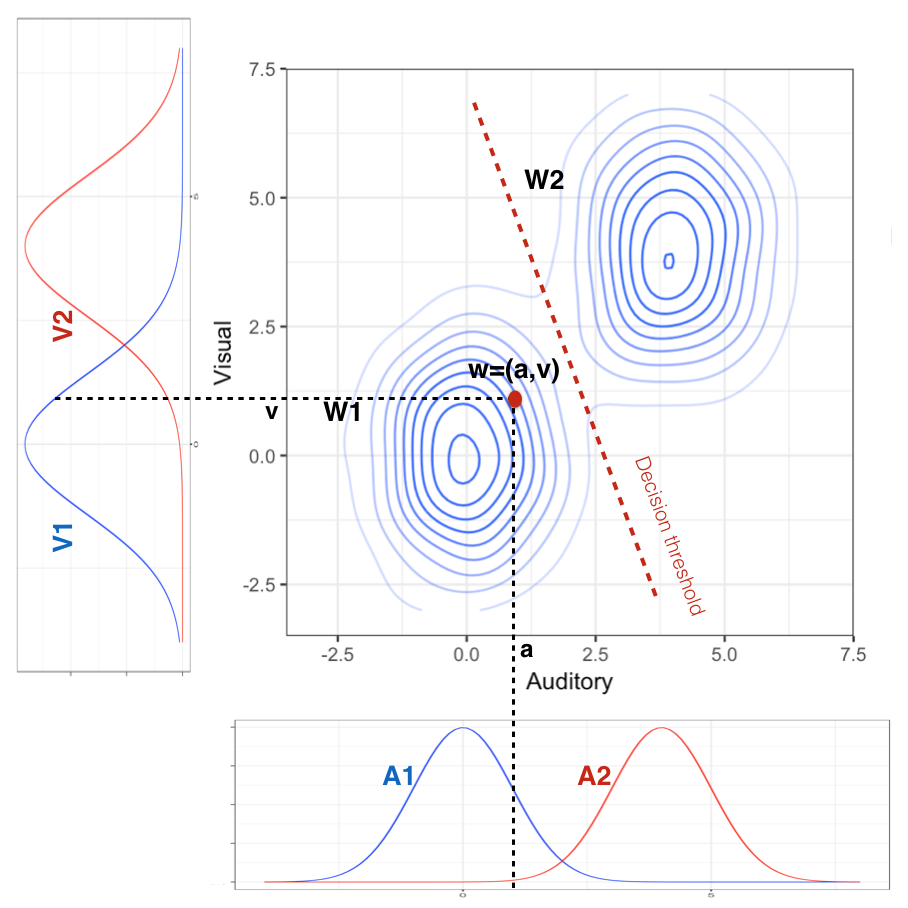
\includegraphics[width=3.25in]{MyTask.png}
  \caption{Illustration of our model using simulated data. A word category is defined as the joint bivariate distribution of an auditory category (horizontal, bottom panel) and a visual semantic category (vertical, left panel). Upon the presentation of a word token $w$, participants guess whether it is sampled from the word category $W_1$ or from $W_2$. Decision threshold is where the guessing probability is 0.5.}
  \label{fig:space}
\end{figure}

We have two word categories: dog-/aba/ ($W_1$) and cat-/ada/ ($W_2$). Participants can be understood as choosing one of these two word categories (Figure \ref{fig:space}). For an ideal observer, the probability of choosing category 2 when presented with an audio-visual instance $\mathbf{w}=(a,v)$ is the posterior probability of this category:

\begin{equation}
% \small
p(W_2 | \mathbf{w})=\frac{p(\mathbf{w}|W_2)p(W_2)}{p(\mathbf{w}|W_2)p(W_2)+p(\mathbf{w}|W_1)p(W_1)}
\end{equation}

We make the assumption that, given a particular word category, the auditory and visual tokens are independent:

\begin{equation}
p(\mathbf{w} | W) = p(a,v| W) = p(a| W)p(v| W)
\end{equation}

Under this assumption, the posterior probability reduces to:
\begin{equation}
p(W_2 | \mathbf{w})=\frac{1}{1+(1+\epsilon)\exp(\beta_0+\beta_aa+\beta_vv)}
\label{eq:pred}
\end{equation}

\noindent with $\beta_a=\frac{\mu_{A1}-\mu_{A2}}{\sigma^2_{A}}$,
$\beta_v=\frac{\mu_{V1}-\mu_{V2}}{\sigma^2_{V}}$,
$\beta_0=\frac{\mu^2_{A2}-\mu^2_{A1}}{2\sigma^2_{A}}+\frac{\mu^2_{V2}-\mu^2_{V1}}{2\sigma^2_{V}}$
and $1+\epsilon=\frac{p(W_1)}{p(W_2)}$ is the proportion of the prior probabilities. If the identity of word categories is randomized, and if $W_1$ is the target, then $\epsilon$ measures a response bias to ``same'' if $\epsilon > 0 $, and a response bias to ``different'' if $\epsilon < 0 $.

In sum, the posterior \ref{eq:pred} provides the predictions of ideal observer for how probabilities that characterize uncertainty in each modality can be combined to make categorical decision about bimodal input.


\section{Experiment 1}

In Experiment 1, we test the predictions of the model in the case where uncertainty is due to similar auditory categories, and similar visual categories. Crucially, the similarity is such that the distributions overlap. To simulate such uncertainty in a controlled fashion, we use a continuum along the second formant (F2) linking the words /aba/ and /ada/, and we use a morph that links dogs and cats.

\subsection{Methods}

\subsubsection{Participants}

We recruited a planned sample of 100 participants, recruited from Amazon Mechanical Turk. Only participants with US IP addresses and a task approval rate above 85\% were allowed to participate. They were paid at an hourly rate of \$6/hour. Data were excluded if participants completed the task more than
once (2 participants). Moreover, as specified in the preregistration (\url{https://osf.io/h7mzp/}), participants were excluded if they had less than 50\% accurate responses on the unambiguous training trials (6), and if they reported having experienced a technical problem of any sort during the online experiment (14). The final sample consisted of 76 participants.

\subsubsection{Stimuli}

For  auditory stimuli, we used the continuum introduced in \citeA{vroomen2004}, a 9-point /aba/--/ada/ speech continuum created by varying the frequency of the second (F2) formant in equal steps. We selected 5 equally spaced points from the original continuum by keeping the end-points (prototypes) 1 and 9, as well as points 3, 5, and 7 along the continuum. For visual stimuli, we used a morph continuum introduced in \citeA{freedman2001}: a continuous set of images was generated from three cat prototypes and three dog prototypes. From the original 14 points, we selected 5 points as follows: we kept the item that seemed most ambiguous (point 8), the 2 preceding points (i.e., 7 and 6) and the 2 following points (i.e., 9 and 10). The 6 and 10 points along the morph were quite distinguishable, and we took them to be our prototypes.

 % (Figure \ref{fig:morph})
%
% \begin{figure}[tp]
% \centering
% 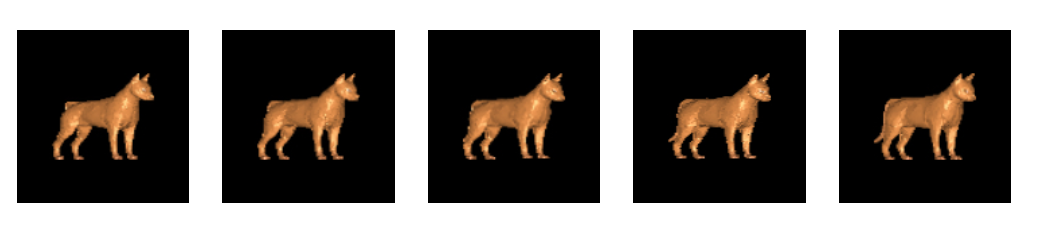
\includegraphics[width=0.4\textwidth]{morph.png}
% \caption{Visual stimuli for our experiments.}
% \label{fig:morph}
% \end{figure}

\subsubsection{Design and Procedure}

We told participants that an alien was naming two objects: a dog, called /aba/ in the alien language, and a cat, called /ada/. In each trial, we presented the first object (the target) on the left side of the screen simultaneously with the corresponding sound. The target was always the same (e.g., dog-/aba/). The second sound-object pair (the test) followed on the other side of the screen after 500ms and varied in its category membership. For both the target and the test, visual stimuli were present for the duration of the sound clip ($\sim$800ms). We instructed participants to press ``S'' for same if they thought the alien was naming another dog-/aba/, and ``D'' for different if they thought the alien was naming a cat-/ada/. For each participant, we randomized the sound-object mapping as well as the identity of the target.

The first part of the experiment trained participants using only the prototype pictures and the prototype sounds (12 trials, 4 each from the bimodal, audio-only, and visual-only conditions). After completing training, we instructed participants on the structure of the task and encouraged them to base their answers on both the sounds and the pictures (in the bimodal condition). There were a total of 25 possible combinations in the bimodal condition, and 5 in each of the unimodal conditions. Each participant saw each possible trial twice, for a total of 70 trials/participant. Trials were blocked by condition and blocks were presented in random order.
% We designed the experiment to take between 10 to 15 minutes to complete.

\begin{figure}
\centering
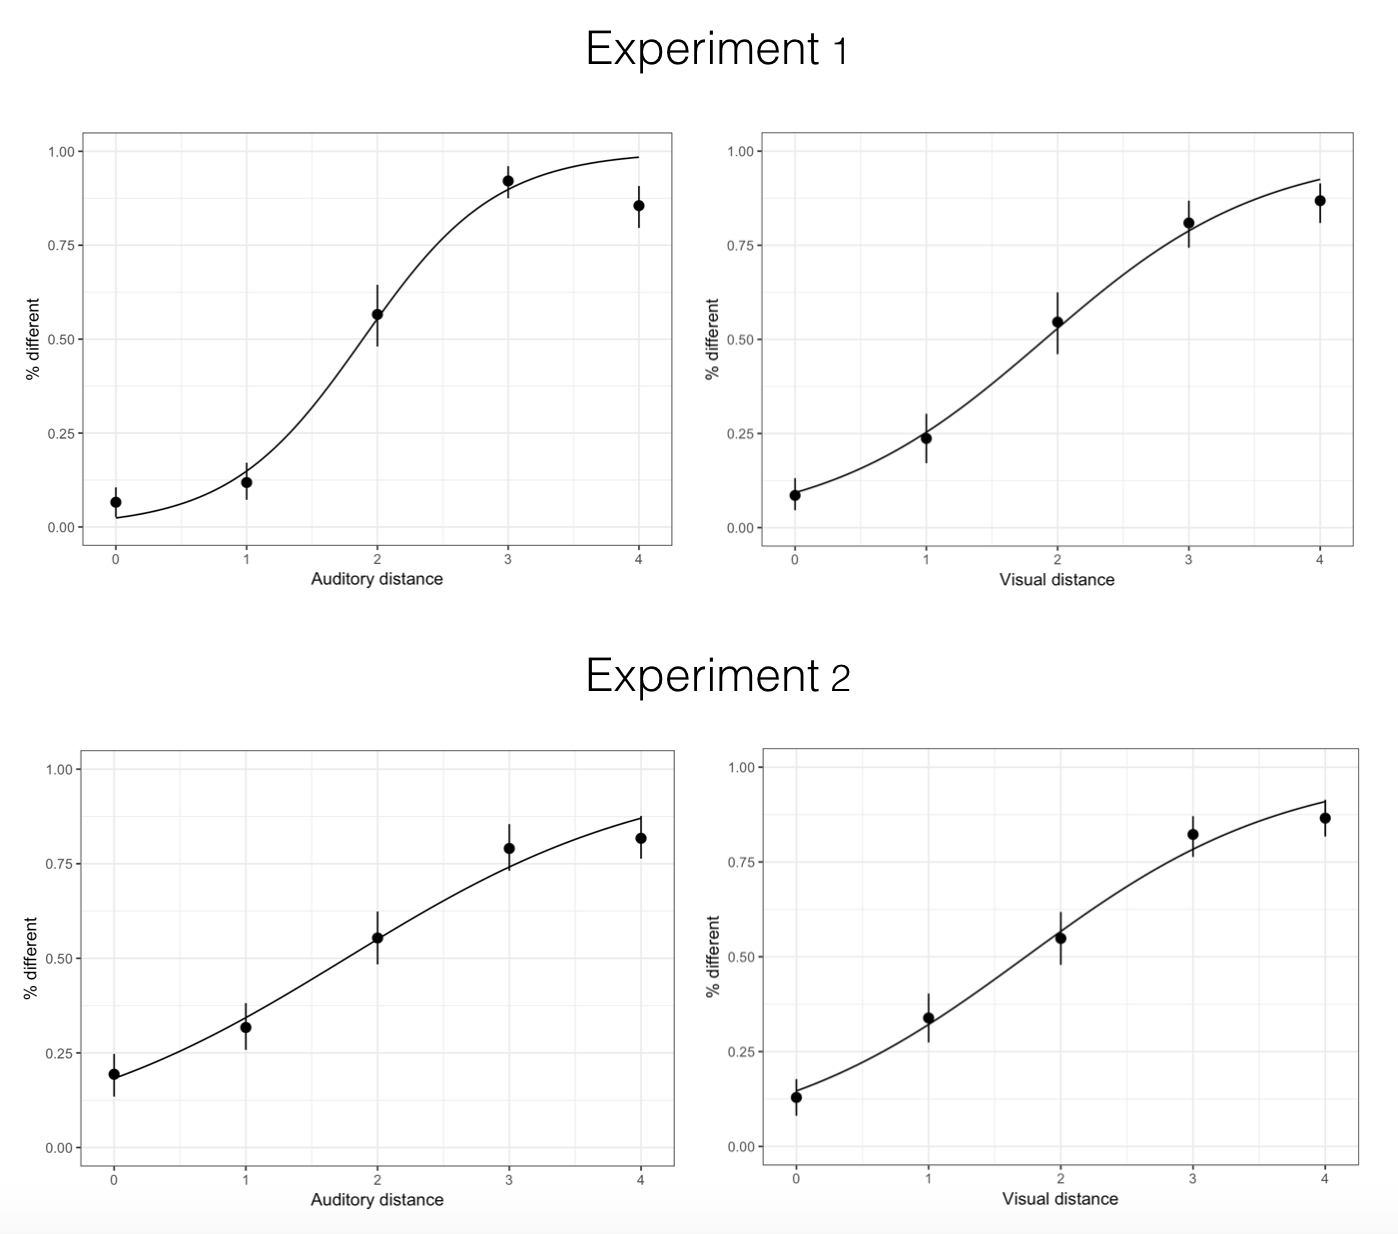
\includegraphics[width=3.25in]{unimodal.png}
\caption{Average human responses in the auditory-only condition (left), and visual-only condition (right). Error bars are 95\% confidence intervals. Solid lines represent unimodal logistic fits.}
\label{fig:unimodal}
\end{figure}


\subsection{Results}
%
% \begin{figure}[h]
% \centering
% 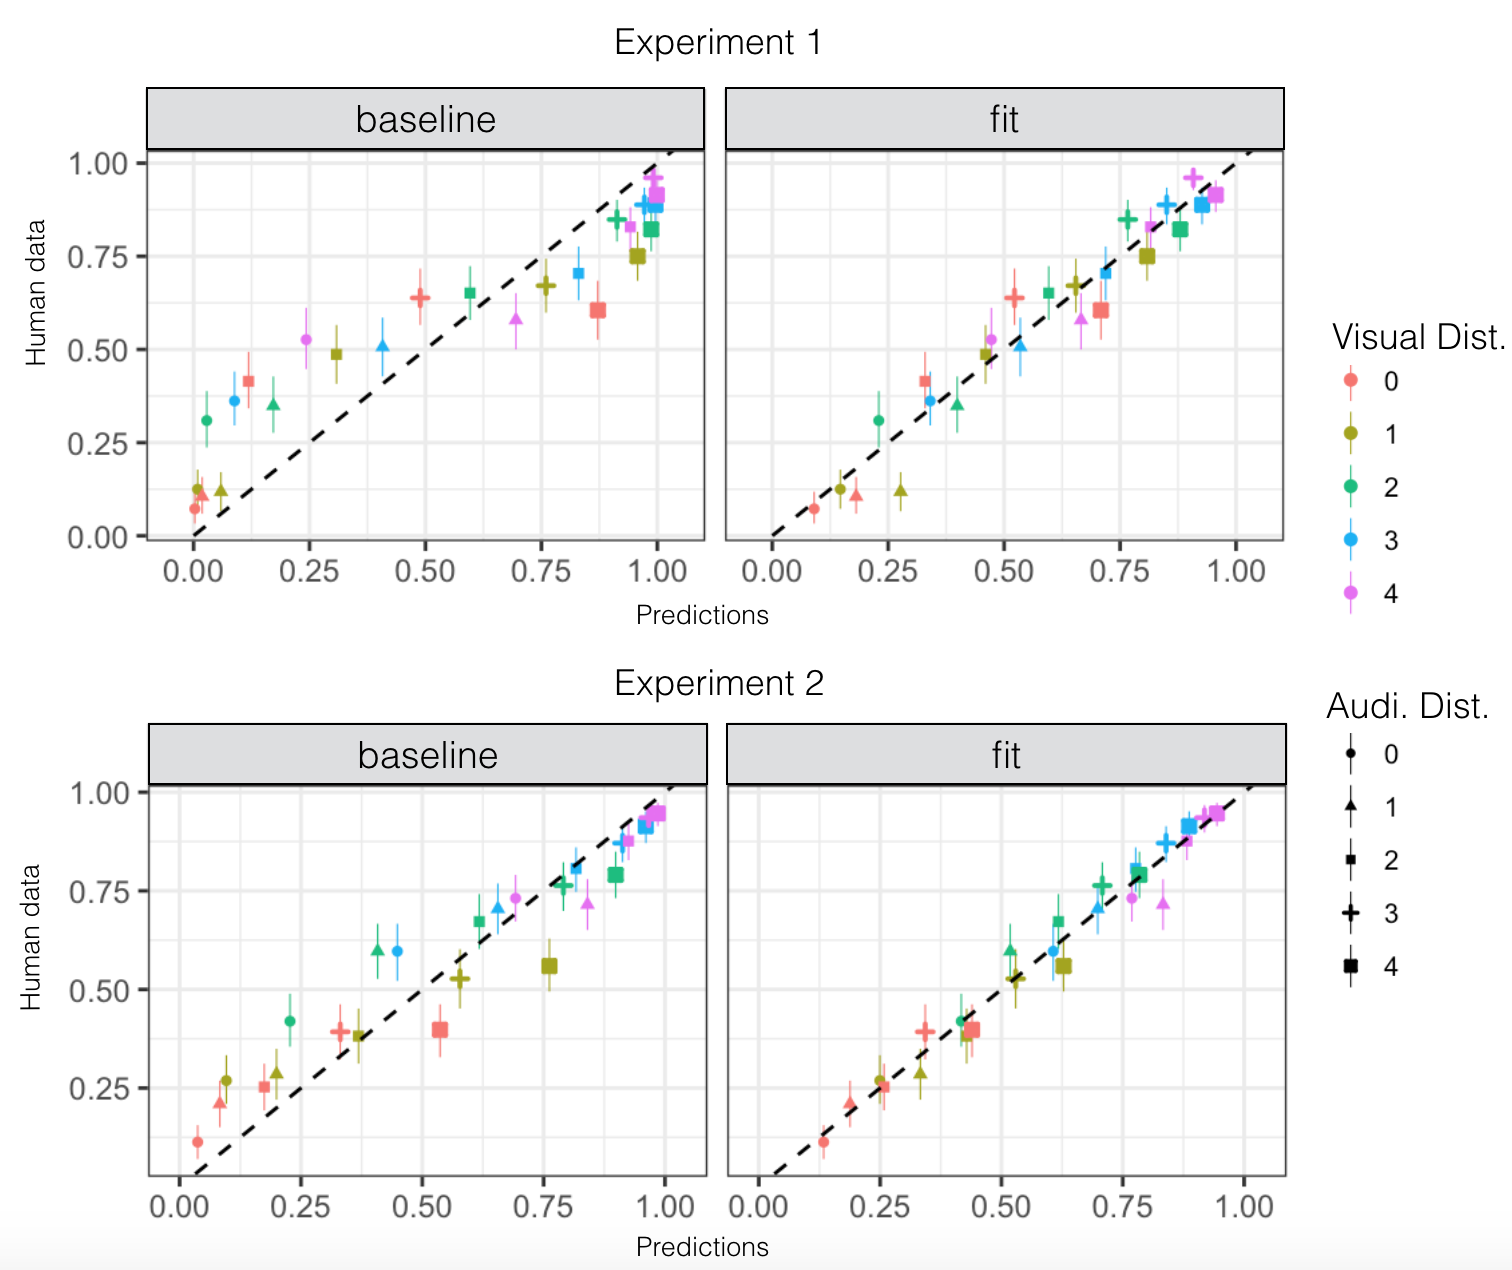
\includegraphics[width=3.25in\textwidth]{correlation.png}
% \caption{Human responses vs. the ideal observer predictions. Error bars are 95\% confidence intervals. In experiment 1, the ideal observer and the fit explained 89\%, and 94\% of total variance, respectively. In experiment 2, the ideal observer and the fit explained 91\%, and 97\% of total variance, respectively}
% \label{fig:corr}
% \end{figure}

\begin{figure*}[t]
\centering
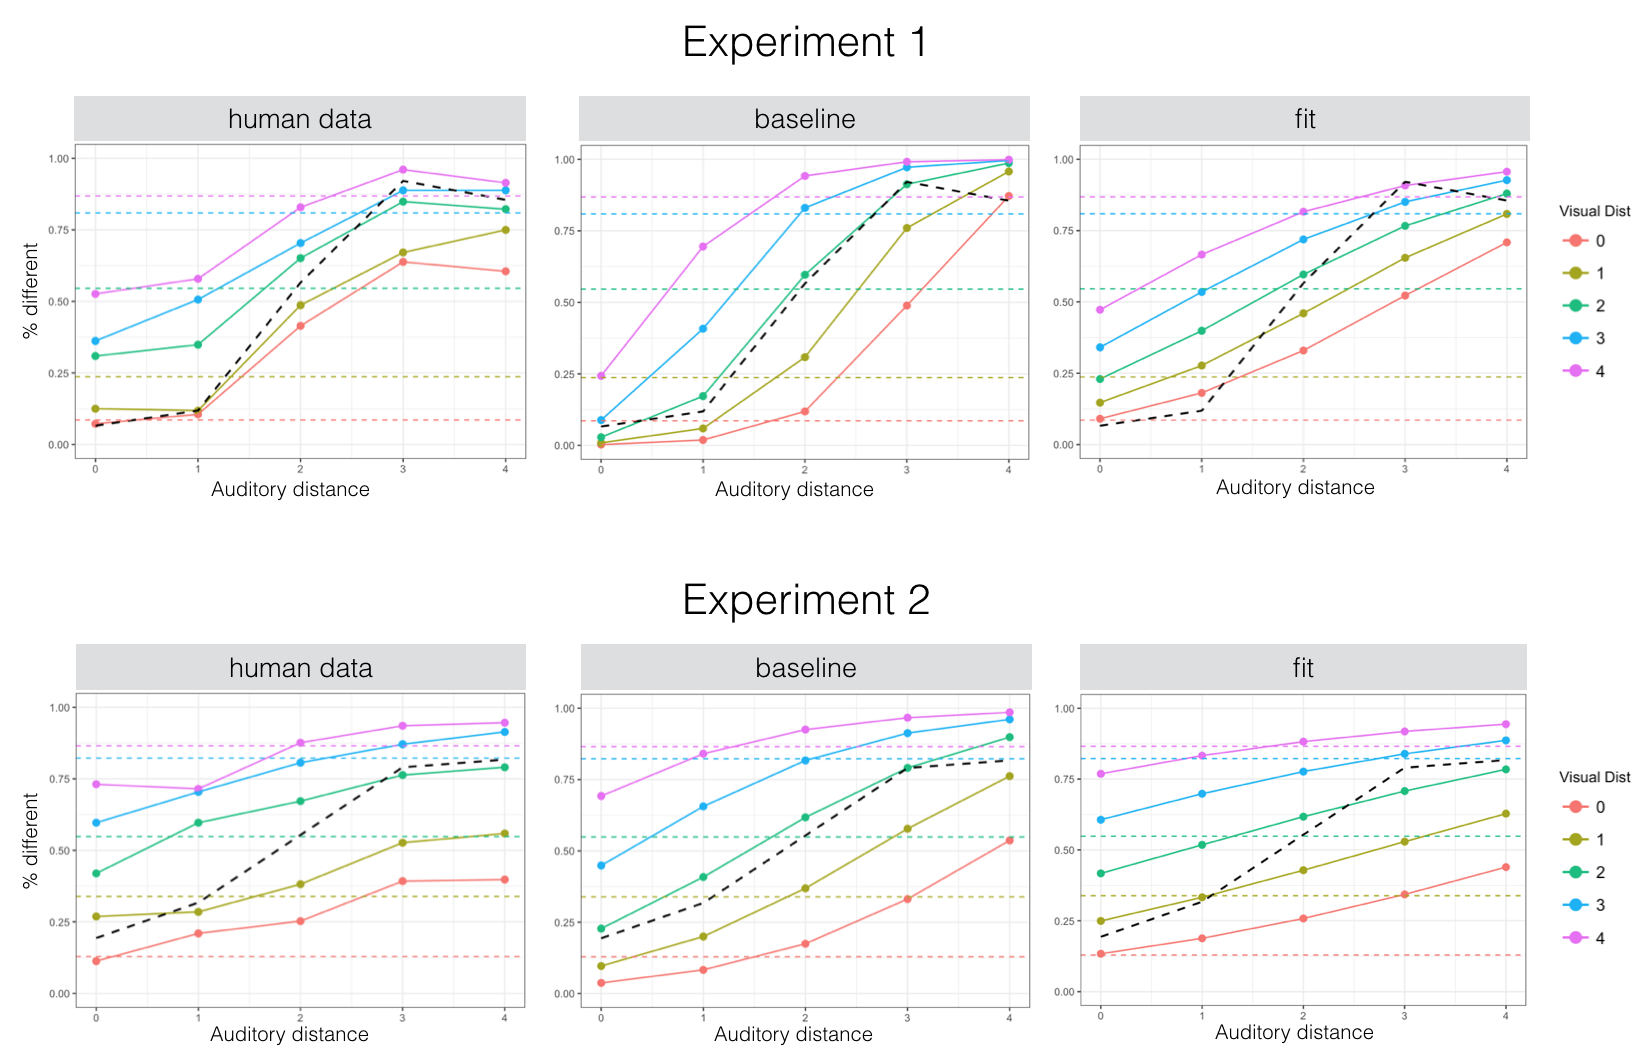
\includegraphics[width=.83\textwidth]{Exp.png}
\caption{Proportion of ``different'' judgments as a function of auditory distance. Solid lines represent average human responses (left), predictions of the ideal observer (middle), and the bimodal fit (left). Dashed lines represent average human responses in the unimodal conditions. Colors represent values in the visual continuum.}
\label{fig:Exp}
% \vspace{10ex}
\end{figure*}

% Let's take the auditory-only case as an example,
\subsubsection{Unimodal conditions} this is the case where the pictures were hidden, or where the sounds were muted.
Average categorization judgments and fits are shown in Figure \ref{fig:unimodal}. Auditory judgements were somewhat sharper and more pronounced than visual judgments. The fit was done as follows. For an ideal recognizer, the probability of choosing category 2 (that is, to answer ``different'') when presented with an audio instance $a$, is the posterior probability of this category $p(A_2|a)$. If we assume that both categories have equal variances, the posterior probability reduces to:

\begin{equation}
p(A_2 | a)=\frac{1}{1+(1+\epsilon_A)\exp(\beta_{a0}+\beta_aa)}
\end{equation}

\noindent with $\beta_a=\frac{\mu_{A_1}-\mu_{A_2}}{\sigma^2_{A}}$ and  $\beta_{a0}=\frac{\mu^2_{A_2}-\mu^2_{A_1}}{2\sigma^2_{A}}$. $\epsilon_A$ is the response bias in the auditory-only trials.

For this model (as well all other models), we fixed the values of the means to be the end-points of the corresponding continuum: $\mu_{A1}=0$ and $\mu_{A2}=4$ (and similarly $\mu_{V1}=0$, and $\mu_{V2}=4$). To determine the values of the bias and the variance, we fit a model for each modality, collapsed across participants. For the auditory modality, we obtained $\epsilon_A=-0.20$ and $\sigma^2_A=2.04$. For the visual modality, we obtained $\epsilon_V=-0.11$ and $\sigma^2_V=3.34$.

\subsubsection{Bimodal condition}
We fit a model to human responses in the bimodal condition, collapsed across participants, finding $\epsilon=-0.32$, $\sigma^2_{Ab}=5.00$ and $\sigma^2_{Vb}=7.27$. The fit explained XX of the variance.

\subsubsection{Ideal observer model}

We derived the predictions of the ideal observer model by using the values of the variances derived from the unimodal conditions, and the response bias derived from the bimodal condition, and by substituting these values into the expression of the posterior in Eq.~\ref{eq:pred}.
Figure \ref{fig:Exp} shows participants' responses in the bimodal condition (left), as well as the prediction of the ideal observer (middle), and the bimodal fit models (right).

\subsubsection{Response bias}

We found negative values in all response bias terms, which suggests a general bias toward answering ``different.''  This bias is probably due to the categorical nature of our same-different task: when two items are ambiguous but perceptually different, this could cause a slight preference for ``different'' over ``same''.

\subsubsection{Modality preferences}

We next analyzed whether there was a preference for one or the other modality when making decisions in the bimodal condition, beyond that explained by the variance in categories implied by the unimodal responses. This preference would manifest as a deviation from the decision threshold predicted by the ideal observer model. The decision threshold is defined as the set of values in the audio-visual space along which the posterior (Eq.~\ref{eq:pred}) is equal to 0.5. The decision threshold takes the following form:

\begin{equation}
v=-\frac{\sigma^2_V}{\sigma^2_A}a+v_0
\label{eq:threshold}
\end{equation}

If the slope derived from the bimodal fit is greater than the slope of the ideal observer, this finding would suggest a general preference for the auditory modality (similarly, a smaller slope would suggest a preference for the visual modality). The limit cases are when there is exclusive reliance on the auditory cue (a vertical line), and where there is exclusive reliance on the visual (a horizontal line). Figure \ref{fig:pref} (top left) shows the decision threshold in the audio-visual space with a constant intercept; the fit to human data  (solid black line) was very close to the ideal observer threshold (red line). Non-parametric resampling of the data showed no evidence of a deviation from the slope of the ideal observer (\ref{fig:pref}, bottom left).

\subsection{Discussion}

Qualitatively, participants' judgments were similar to the predictions of the ideal observer model (remember that the latter was obtained by optimally combining fits to the unimodal data). Consider, for example, the contrast between the auditory-only case (dashed black line in Figure \ref{fig:Exp}, top left) and the bimodal case (solid colored lines).  Higher certainty in the visual modality generally influenced responses, with greater visual distance leading to more ``different'' ratings and less visual distance leading to more ``same'' ratings. Similar observations can be made about the contrast between the visual-only case and the bimodal case.

Overall, we found that the ideal observer model explained much of the variance in judgments ($r^2=0.89$). But although we see a qualitative resemblance between human data and the model, there were quantitative differences. For example, model predictions were more influenced by the visual modality at the auditory midpoint (the point of highest uncertainty) than human judgements, and were more compressed at the endpoints (the points of lowest uncertainty).

Formally, there was an increase in the value of the variance associated with each modality. Whereas the ideal observer model predicted the weights to be proportional to $1/\sigma^2_{A}$ and $1/\sigma^2_{V}$, for the auditory and the visual modalities, respectively (see expression \ref{eq:pred}), the fit to human data suggested that the real weights were proportional to $1/\sigma^2_{Ab}$ and $1/\sigma^2_{Vb}$. Our analysis of modality preference showed that the relative values of these variances were almost the same (Figure \ref{fig:pref}, left). Thus, 1) the bimodal presentation caused reliance on both modalities to decrease, and 2) this decrease did not affect the relative weighting of both modalities, i.e., participants were weighting modalities according to their relative reliability. The latter explains the qualitative resemblance between the predictions of the ideal observer and human data, and the former explains the quantitative discrepancy.

% (i.e., $\frac{\sigma^2_V}{\sigma^2_A}$ vs. $\frac{\sigma^2_{Vb}}{\sigma^2_{Ab}}$)

In sum, we found that participants followed the ideal observer model in that they weighted modalities according to their reliabilities. In real life, however, tokens can undergo distortions due to noisy factors in the environment. In Experiment 2, we explore this additional level of uncertainty.

\section{Experiment 2}

Imagine that the speaker generates a target production $t$ from an auditory category
$t | A \sim N(\mu_{A}, \sigma^2_{A})$. In Experiment 1, we assumed that the observed could directly retrieve this production token. But if the observer is in a noisy environment, they do not hear exactly this produced target, but the target perturbed by noise, which we assume, following \citeA{feldman2009}, that it is normally distributed: $a | t \sim N(t, \sigma^2_{N})$. When we integrate over $t$, we get:

\begin{equation}
a | A \sim N(\mu_{A}, \sigma^2_{A}+\sigma^2_{N})
\end{equation}

In this experiment, we explored the effect of this added noise\footnote{Note that we are considering environmental noise, which is different from the noise inherent to perception.} on performance in our task. We tested a case where one modality was ambiguous and noisy (auditory), and where the other modality was ambiguous but not noisy (visual). We were interested to know if participants would treat this new source of uncertainty as predicted by the ideal observer model, and whether noise in one modality would lead to some systematic preference for the non-noisy modality.

\subsection{Methods}

\subsubsection{Participants}

A planned sample of 100 participants was recruited online through Amazon Mechanical Turk. We used the same exclusion criteria as in the previous experiment; the final sample consisted of 93 participants.

\subsubsection{Stimuli and Procedure}

We used the same visual stimuli as in Experiment 1. We also used the same auditory stimuli, but we convolved each item with Brown noise of amplitude 1 using the audio editor Audacity (2.1.2).  The signal-to-noise ratio was XXX dB. The procedure was exactly the same as in the previous experiment, except that test stimuli were presented with the new noisy auditory stimuli.

\subsection{Results}

\subsubsection{Unimodal conditions}

We fit a model for each modality, collapsed across participants. For the auditory modality, our parameter estimates were $\epsilon_A=-0.18$ and $\sigma^2_A+\sigma^2_N=4.70$. For the visual modality, we found $\epsilon_V=-0.24$ and $\sigma^2_V=3.93$.  Figure \ref{fig:unimodal} (bottom) shows responses in the unimodal conditions as well as the unimodal fits. In contrast to Experiment 1, auditory responses were flatter (showing more uncertainty).

\subsubsection{Bimodal condition}

We fit a model to human responses in the bimodal condition, collapsed across participants. We estimated $\epsilon=-0.38$, $\sigma^2_{Vb}=5.21$, and  $\sigma^2_{Ab}+\sigma^2_{Nb}=9.84$.

\subsubsection{ideal observer model}

We generated the predictions of the ideal observer model by using the values of the variances derived from the unimodal conditions, and the response bias derived from the bimodal condition, and by substituting these values into the expression of the posterior in Eq.~\ref{eq:pred}.
Results are shown in Figure \ref{fig:Exp} (bottom).

\subsubsection{Modality preferences}

Participants' decision threshold suggested a preference for the visual modality (the non-noisy modality). Indeed non-parametric resampling of the data showed a decrease in the value of the slope (\ref{fig:pref}, right).

\subsection{Discussion}

\begin{figure}[h]
\centering
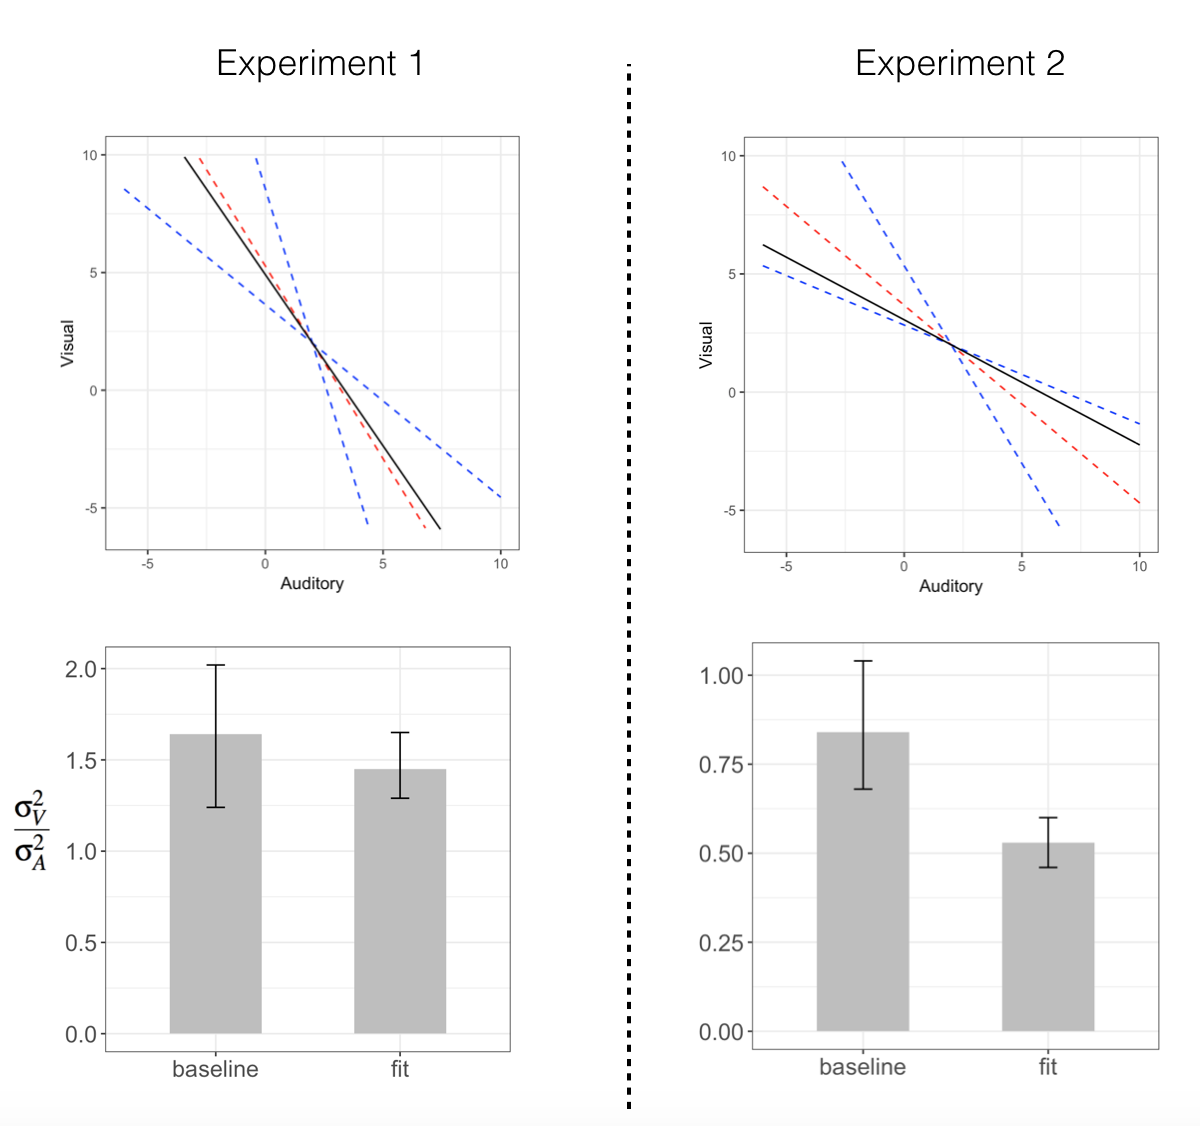
\includegraphics[width=0.4\textwidth]{preference.png}
\caption{Top: decision thresholds in the audio-visual space. Red dotted line is the prediction of the ideal observer. Blue dotted lines are cases where modality preference is twice as strong as the ideal observer. Solid line is the threshold derived from human data. Bottom: comparison of the threshold slope between the ideal observer and the fit to human data. Error bars are 95\% confidence intervals computed via non-parametric bootstrap.}
\label{fig:pref}
\end{figure}

We found, similar to Experiment 1, that participants generally showed qualitative patterns similar to the ideal observer model ($r^2 = .91$). But we also found a similar discrepancy at the quantitative level. The ideal observer model predicted the modality weights to be proportional to $1/(\sigma^2_{A}+\sigma^2_{N})$ and $1/\sigma^2_{V}$, for the auditory and the visual modalities, respectively. The fit to human data suggested that the empirical weights were proportional to $1/\sigma^2_{Ab}$ and $1/\sigma^2_{Vb}$. An interesting difference with Experiment 1, however, was that participants had a clear preference for the non-noisy modality, as the values of the relative variances were different (Figure \ref{fig:pref}, right). This preference affected the relative weighting, where, contrary to Experiment 1, the visual modality had greater weight than what could be expected from its relative reliability alone.
% $\frac{\sigma^2_V}{\sigma^2_A + \sigma^2_N}$ vs. $\frac{\sigma^2_{Vb}}{\sigma^2_{Ab}}$


It is important to understand that this preference was not the mere consequence of the added noise increasing the variance of the auditory modality, since this increase was already accounted for in the ideal observer model. The preference was, rather, a form of over-reliance on the visual modality.

\section{General Discussion}

Understanding language requires both the ability to integrate multi-modal input, and the ability to deal with uncertainty. In this work, we explored a case where both abilities were at play. We studied the case of identifying a word when both its form (auditory) and its referent (visual) were ambiguous with respect to their category membership (Experiment 1), and when the form was perturbed with additional noise (Experiment 2). We introduced a model that instantiated an ideal observer, predicting how information from each modality could be combined in an optimal way. In both experiments, participants showed the qualitative patterns of the ideal observer.

There were, however, quantitative differences. Audio-visual presentation caused the reliance on both modalities to decrease to a lower extent than the ideal observer model expected. One possbible explanation is that this phenomenon was caused by the arbitrary nature of the form-meaning mapping. Previous studies suggest that while redundant multi-modal information improves performance (e.g., determining the frequency of a bouncing ball from visual and auditory cues), arbitrary mappings generally tends to hinder performance \cite<for review, see>{robinson2010}.
% Or perhaps the ideal model failed to capture some other features of multi-modal integration.
% Further work is needed to understand this result.

Interestingly, however, in Experiment 1 this decrease in reliance (or the increase in variance) occurred at a similar rate for both the auditory and the visual modality, and thus, it did not affect their relative weighting. The latter was primarily determined by informational reliability. Only when we intervened by adding  noise to one modality in Experiment 2, did participants show a systematic preference for the non-noisy modality. One possible explanation for this preference could be that people do not combine cross-modal uncertainties of a similar kind (e.g., ambiguity in both modalities) in the same way they would combine uncertainties of different kinds (e.g., ambiguity in one modality and noise in the other).
% Further work is needed to determine the extent to which this is the case.

Overall, in both Experiments, the majority of the variance could be explained by an ideal observer that combined multi-modal information optimally. In the light of this main result, we can revisit some previous findings in the literature. For instance, \citeA{sloutsky2003} reported a dominance for the auditory modality in children. This dominance disappear or reverses in adults. Could this developmental difference be driven by changes in the intrinsic relative reliability of modalities across development? More work is needed to carefully examine this (and other) speculations, and more generally, to determine the extent to which the optimal combination account helps us better understand the mechanisms of word precessing and learning.

\bibliographystyle{apacite}

\setlength{\bibleftmargin}{.125in}
\setlength{\bibindent}{-\bibleftmargin}

\bibliography{CogSci_Template}

\end{document}
